\clearpage
\hypersetup{pageanchor=false}
\setcounter{page}{1}
\maketitlesupplementary

\section{Semantic Affinity Routing Analysis}
Quantitative analysis of the utilization of Mixture of Experts for heterogeneous inputs reveals a fair utilization of Mixture of Experts. Analysis of the heatmap for activation of the model and attention for the expert map reveals that Semantic Affinity Routing (SAR) achieves a structured allocation of tokens to the experts, ensuring that there is no routing collapse, which is a common failure mode for sparse Mixture of Experts.

All visualizations for the routing were produced using the $GlaS$ test $A$ set~\cite{sirinukunwattana2016glandsegmentationcolonhistology} with the SAGE-ConvNeXt+ViT-UNet model and $K = 4$.


\begin{figure}[H]
    \centering
    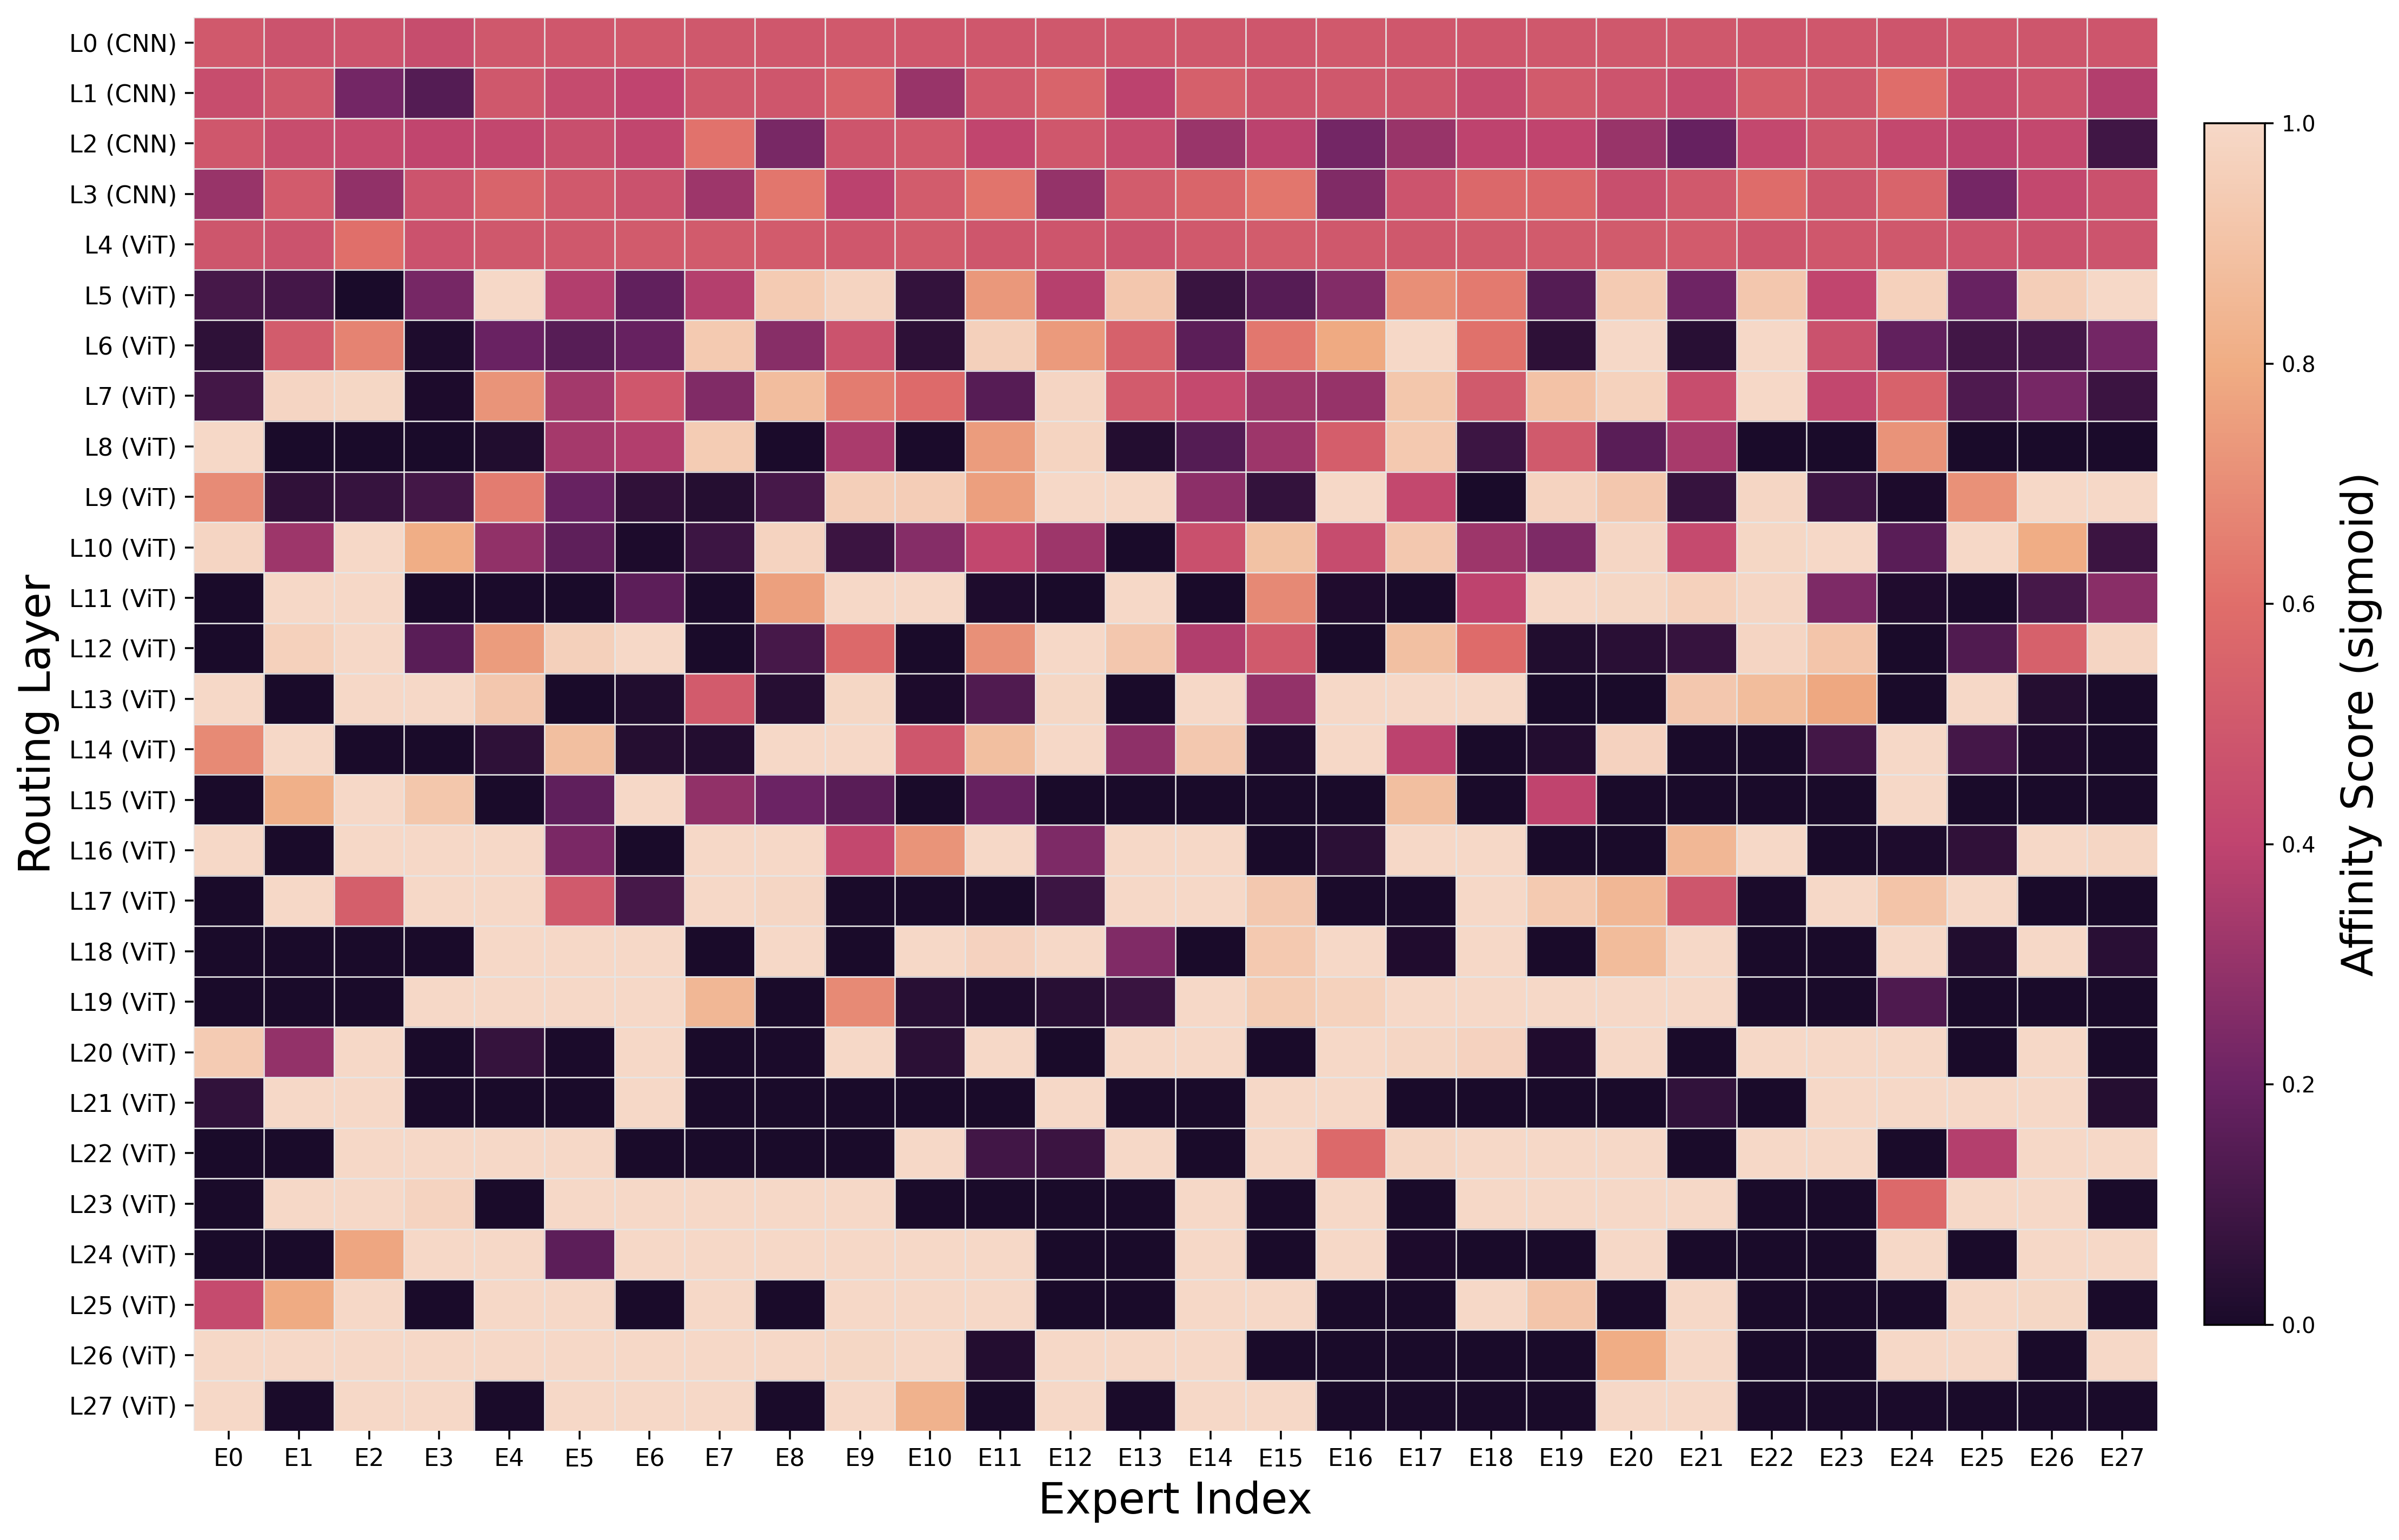
\includegraphics[width=\linewidth]{figs/testA_1_affinity_heatmap.png}
    \caption{
        \textbf{Normalized affinity score heatmap.} The visualization shows the normalized affinity scores, which are the gating probabilities per expert per layer, with a color map ranging from red (low affinity) to dark green (high affinity). The rows in this heatmap represent the model's layer, where $L0$ to $L3$ represent the CNN layers, followed by $L4$ to $L27$, which represent the Vision Transformer layers. The columns represent the 28 experts in the expert pool, where $E0$ to $E27$ represent each individual expert.}
    \label{fig:affinity}
\end{figure}

\begin{figure} [t]
    \centering
    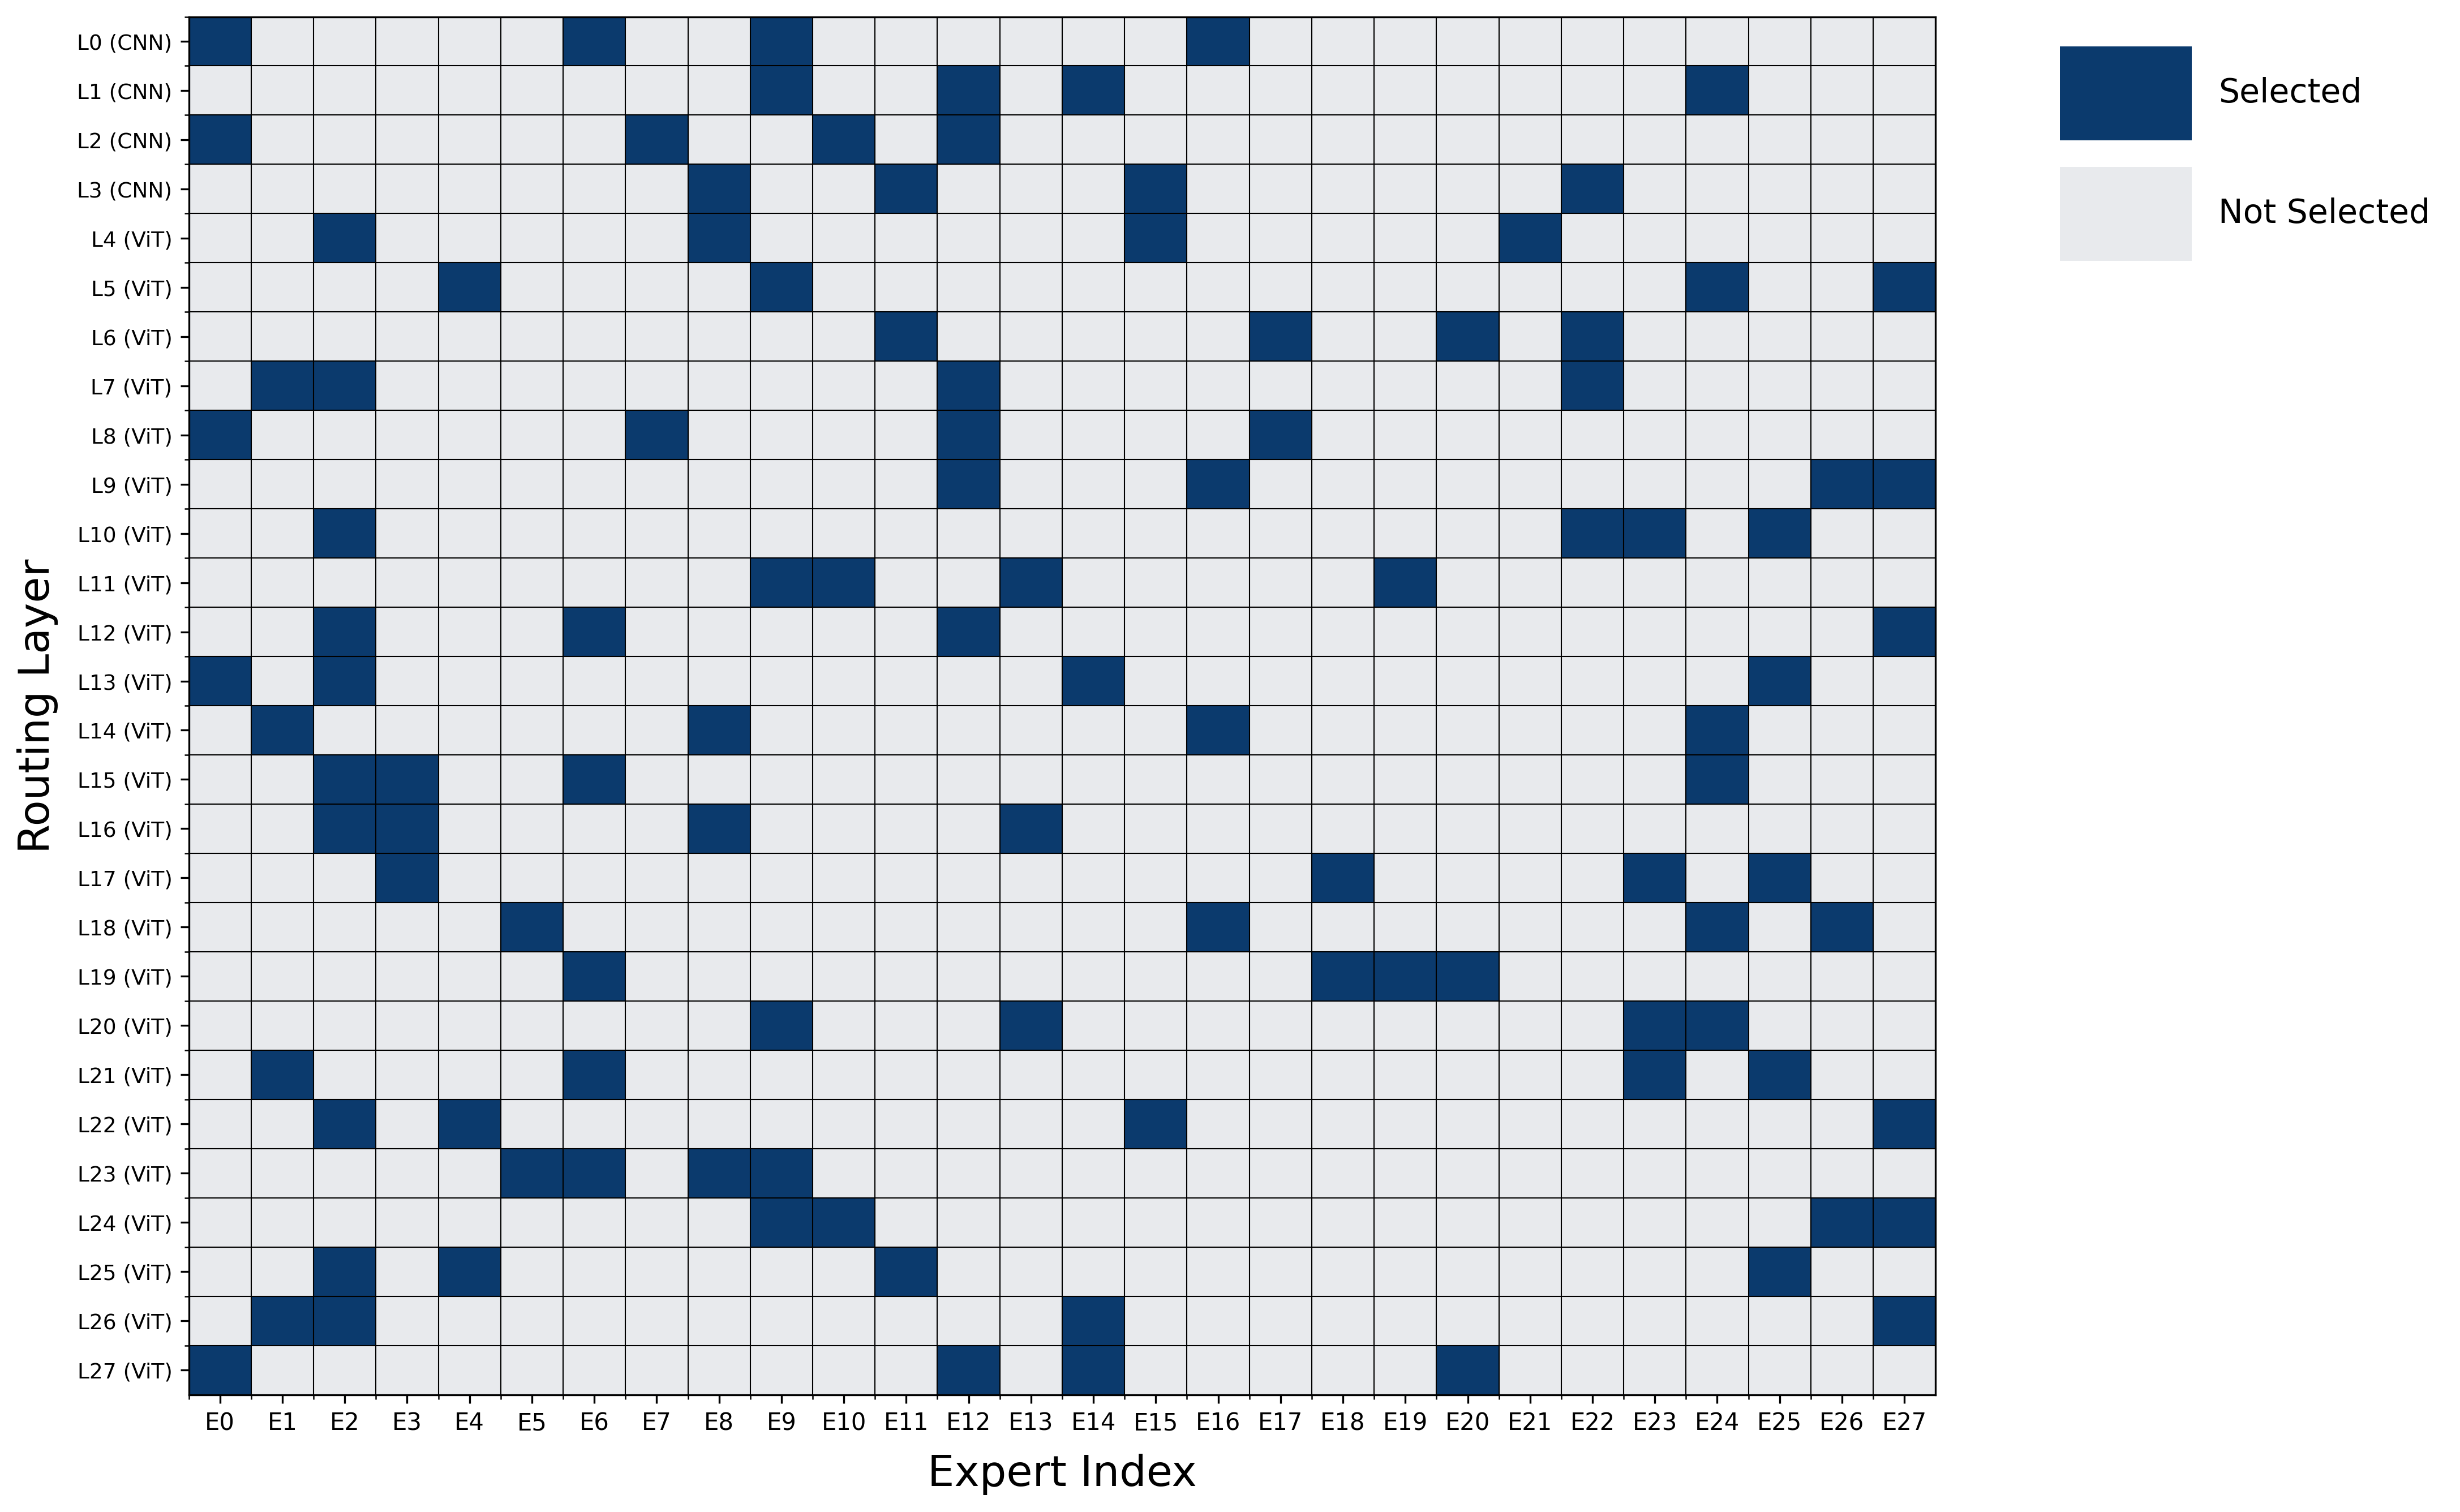
\includegraphics[width=\linewidth]{figs/testA_1_routing_decision_map.png}
    \caption{\textbf{Top-$K$ activation map.} The binary heatmap illustrates the routing decisions, where $K$ is equal to 4, across the 28 layers in the model (rows: $L0$ to $L3$, which represent the CNN layers; $L4$ to $L27$, which represent the Vision Transformer layers) and the 28 experts in the shared pool (columns: $E0$ to $E27$). The activation of an expert in the top K, at least for one token in the layer after processing the entire batch, is represented by blue, while empty boxes indicate no activation.}
    \label{fig:routing}
\end{figure}


\begin{figure*}[t]
    \centering
    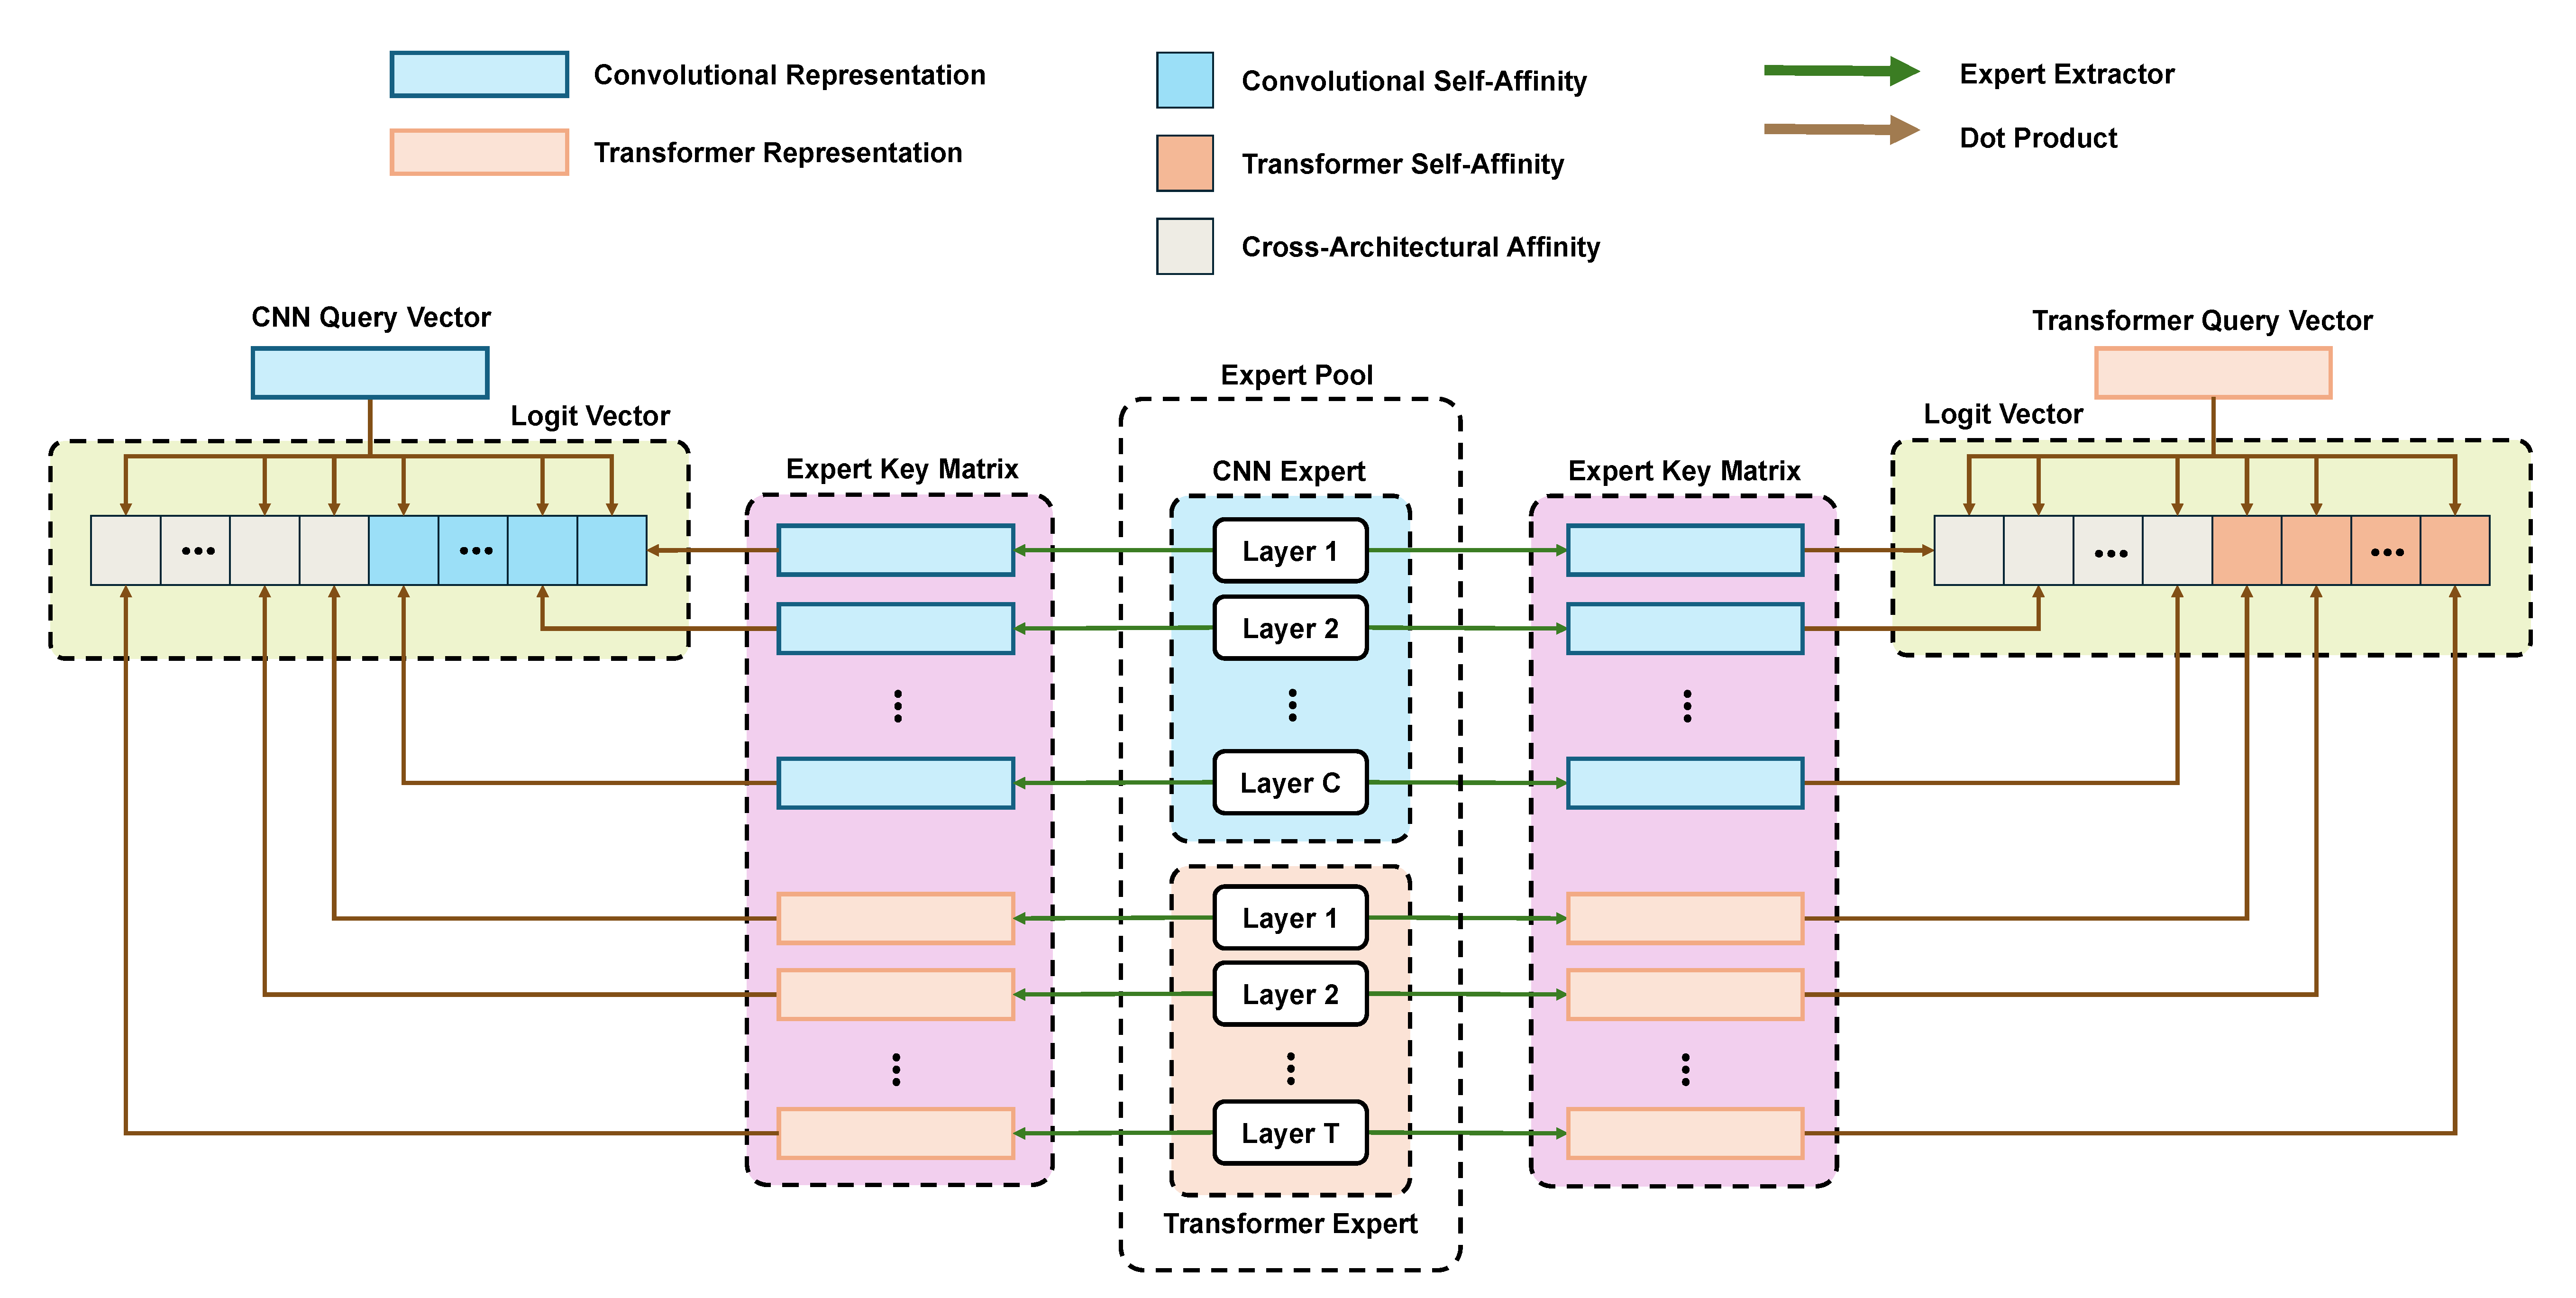
\includegraphics[width=0.9\linewidth]{figs/sar_analysis.pdf}
    \caption{\textbf{Diagnostic view of SAR affinity decomposition.} Given CNN and Transformer query vectors, SAR computes per-expert routing logits by dot-product matching against expert keys extracted from both CNN and Transformer experts. The colored components separate CNN self-affinity, Transformer self-affinity, and cross-architectural affinity contributions, which are aggregated before group-level logit modulation and Top-$K$ selection.}
    \label{fig:sar_supp}
\end{figure*}

Figure~\ref{fig:affinity} shows a non-uniform affinity landscape, indicating layer-dependent expert specialization rather than routing collapse. No expert remains consistently dominant across all layers, and most experts exhibit alternating high/low affinity bands over depth. Stronger contrast appears in the early CNN-to-shallow ViT transition (approximately $L1$--$L4$), while many middle Transformer layers are closer to moderate values, with localized high-affinity reactivation in later layers. Overall, the pattern supports depth-dependent specialization rather than uniform expert usage.



In addition to the global balance observation, Figure~\ref{fig:affinity} reveals clear layer-wise variation. The early CNN and shallow ViT layers show sharper affinity contrast across experts, whereas many middle Transformer layers appear more centered around moderate affinity values. Selected late layers still present localized high-affinity experts, suggesting that specialization is redistributed across depth rather than monotonically increasing toward deeper layers.

Figure~\ref{fig:routing} complements this view by showing activation sparsity patterns per layer at $K=4$. Early CNN layers activate fewer experts per batch, whereas deeper Transformer layers trigger broader expert sets, matching their higher semantic complexity.




Taken together, the two diagnostics indicate that SAR does not behave uniformly across depth: specialization increases in later stages, while early stages remain more shared. This depth-dependent behavior is the key supplementary finding from the routing visualizations.
Figure~\ref{fig:sar_supp} provides a complementary decomposition view, showing how CNN self-affinity, Transformer self-affinity, and cross-architectural affinity jointly contribute to the final Top-$K$ routing decisions.


\section{Group-Level Gate Analysis}
To supplement the mechanistic evidence presented in the main paper, this section visualizes the evolution of the group-level gate $g_s$ on GlaS~\cite{sirinukunwattana2016glandsegmentationcolonhistology} during stage-2 training (Figure~\ref{fig:gs_evolution}). The hierarchical gate's formulation is identical to that in the main paper; the present analysis is restricted to its empirical behavior.

\noindent\textbf{Distribution Shift Across Training.} Figure~\ref{fig:gs_evolution}(a) demonstrates that the final distribution is broader and more polarized than the initial distribution, with substantial mass in both low-$g_s$ and high-$g_s$ regions. This observation indicates that training enhances routing selectivity at the group level, rather than converging to a narrow unimodal regime.

\noindent\textbf{Dynamic Load Balancing.} Figure~\ref{fig:gs_evolution}(b) shows that the mean $g_s$ oscillates around the neutral value ($0.5$): it decreases below $0.5$ during early and mid epochs, increases above $0.5$ in later epochs, and stabilizes near $0.5$ at the end of training. The broad standard deviation band reflects considerable sample-wise heterogeneity throughout training, consistent with input-dependent switching between shared and fine-grained experts.

\noindent\textbf{Architectural Role Specialization.} Figure~\ref{fig:gs_evolution}(c) reveals a consistent architectural gap, with CNN layers exhibiting higher $g_s$ values than Transformer layers.

\begin{figure*}[htp]
\centering
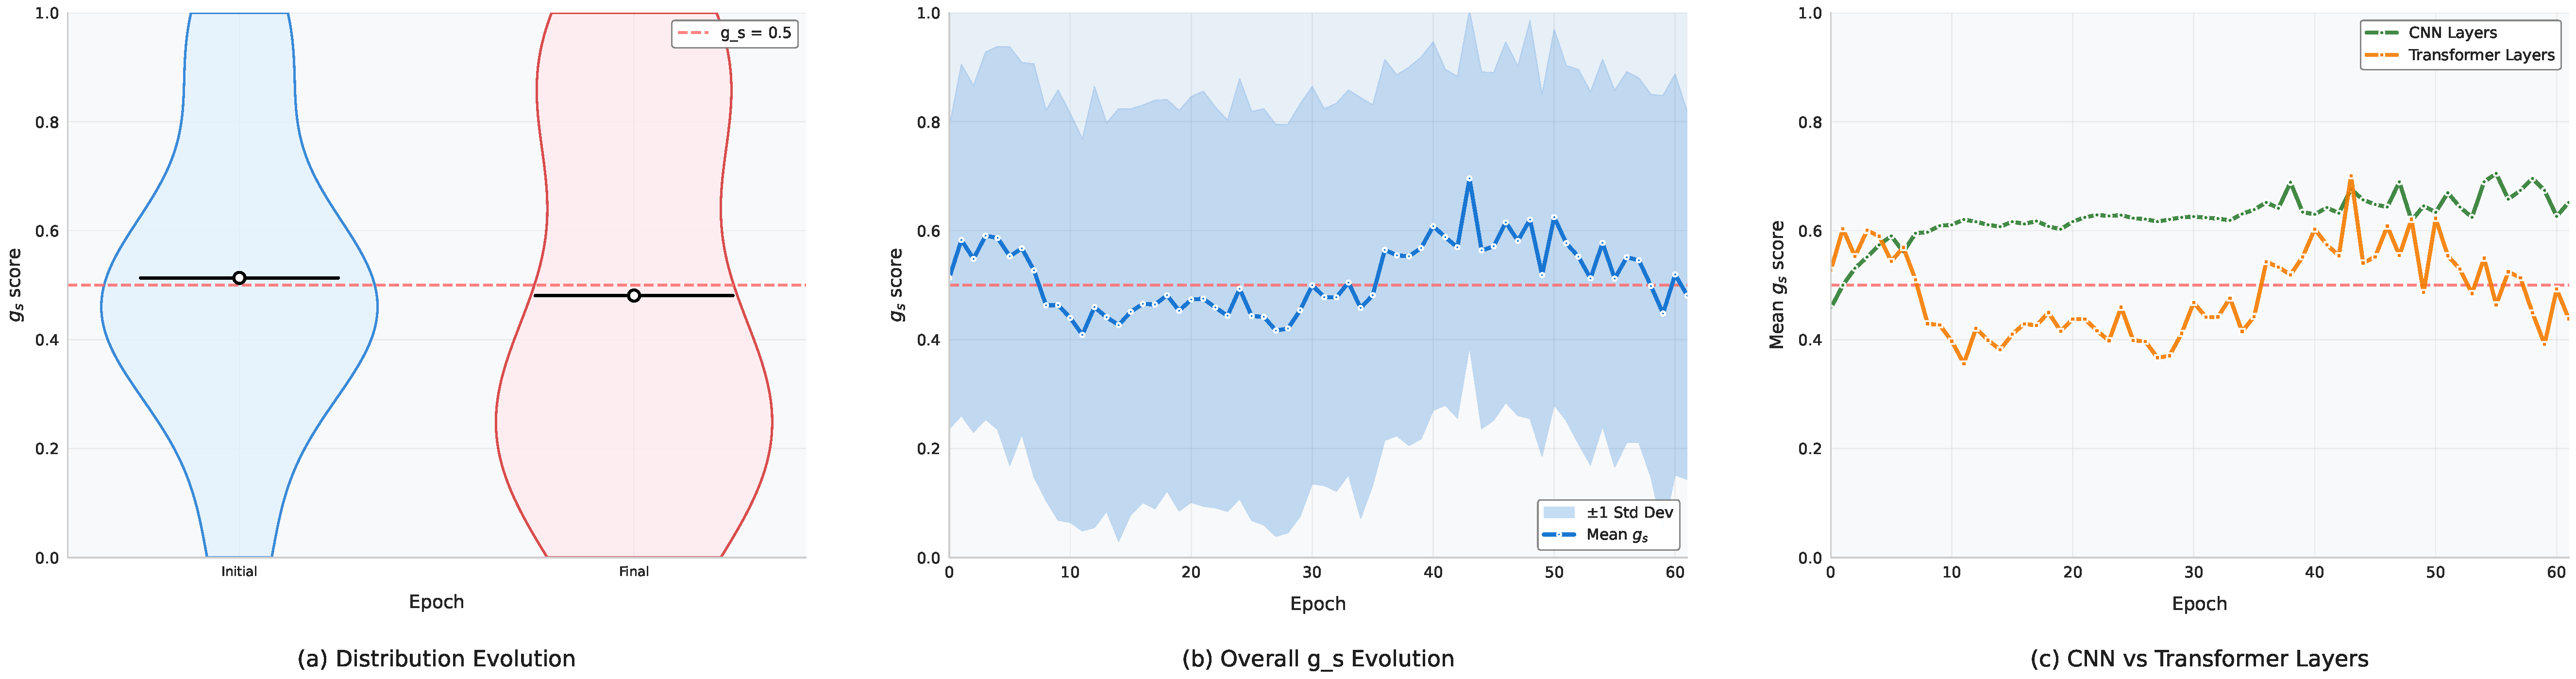
\includegraphics[width=\linewidth]{figs/gs_evolution.pdf}
\caption{\textbf{Group-level gate analysis during training.} The figure illustrates the evolution of $g_s$, where higher values indicate a preference for shared experts and lower values indicate a preference for fine-grained experts. \textbf{(a)} Distribution of $g_s$ at the start and end of training. \textbf{(b)} Mean $g_s$ with standard deviation across 60 epochs, with a neutral reference at $0.5$. \textbf{(c)} Mean $g_s$ by architecture type (CNN versus Transformer), showing that CNN layers remain higher while Transformer layers stay closer to the neutral region.}
\label{fig:gs_evolution}
\end{figure*}

\begin{itemize}
\item \textbf{CNN Layers:} Higher $g_s$ indicates stronger reliance on shared experts, which aligns with the extraction of low-level structural features.

\item \textbf{Transformer Layers:} Lower and more variable $g_s$ values suggest a more frequent preference for fine-grained experts, with periodic shifts back toward neutrality as training advances.

\end{itemize}

These results support the intended division of labor within the hybrid encoder. CNN layers are more oriented toward shared experts, whereas Transformer layers exhibit a tendency toward mixed routing.

\section{Shape-Adapting Hub Analysis}

\begin{figure*}[htp]
\centering

\includegraphics[width=0.9\linewidth]{figs/sahub_2.pdf}
\caption{\textbf{Detailed execution view of the Shape-Adapting Hub (SA-Hub).} The diagram highlights the adaptation path for each expert, which includes input reshaping, expert execution, and output realignment. This process is followed by weighted aggregation across activated experts and gated fusion with the main branch. Blue dashed arrows indicate the flow of shape metadata, while purple arrows represent reshape operations.}
\label{fig:sahub}
\end{figure*}

Figure~\ref{fig:sahub} provides an implementation-level perspective of the SA-Hub and highlights three operational details that are essential for interpreting routing behavior.

First, shape adaptation is performed for each activated expert. Each selected expert receives a dedicated input-side reshape and output-side realignment, enabling heterogeneous expert blocks to operate within the same routed layer.

Second, the diagram distinguishes between expert selection and expert contribution. Top-$K$ routing identifies the active experts, while subsequent weighting and fusion stages determine the extent to which each active expert influences the final representation.

% \begin{figure}[t!]
% \centering

% % ================= Spacing Setup =================
% \newcommand{\gap}{1pt}              % Internal vertical gap
% \setlength{\tabcolsep}{1pt}         % Horizontal gap between columns
% \renewcommand{\arraystretch}{1}

% \newcommand{\imgw}{0.23\textwidth} % Adjusted from 0.18 to 0.23 to better fill the page width with 4 columns

% \resizebox{\linewidth}{!}{%
% \begin{tabular}{@{}p{0.02\textwidth}cccc@{}}
%     & \scriptsize\textbf{(a) Input} &
%     \scriptsize\textbf{(b) SegFormer} &
%     \scriptsize\textbf{(c) EViT-UNet} &
%     \scriptsize\textbf{(d) Ours} \\[4pt]

%     % ================= WSI Sample 1 =================
%     \raisebox{-0.5\totalheight}{\rotatebox{90}{\scriptsize\textbf{WSI Sample 1}}} &
%     \begin{minipage}{\imgw}
%         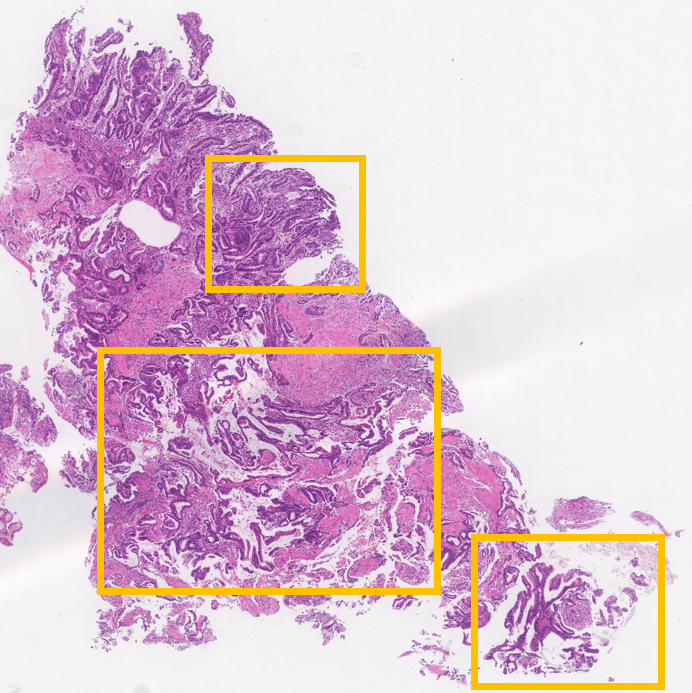
\includegraphics[width=\linewidth]{figs/wsi_img1.png}\\[\gap]
%         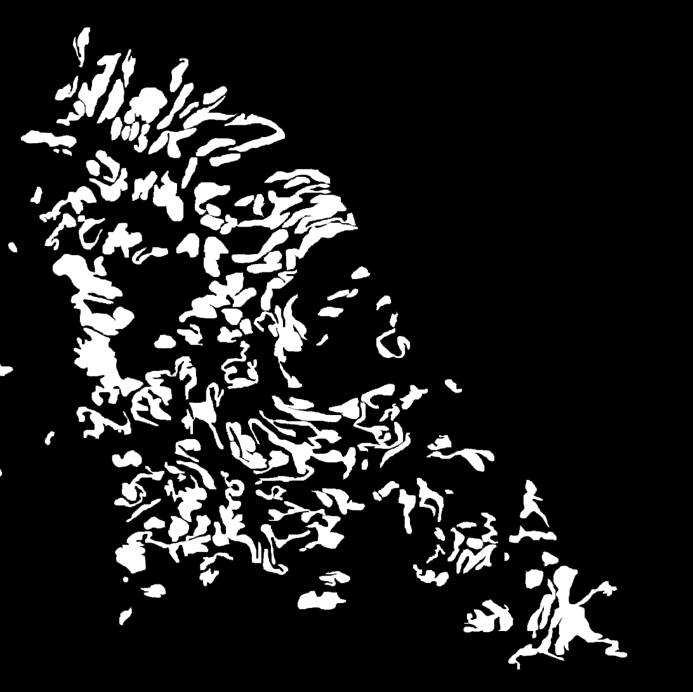
\includegraphics[width=\linewidth]{figs/wsi_gt1.png}
%     \end{minipage} &
%     \begin{minipage}{\imgw}
%         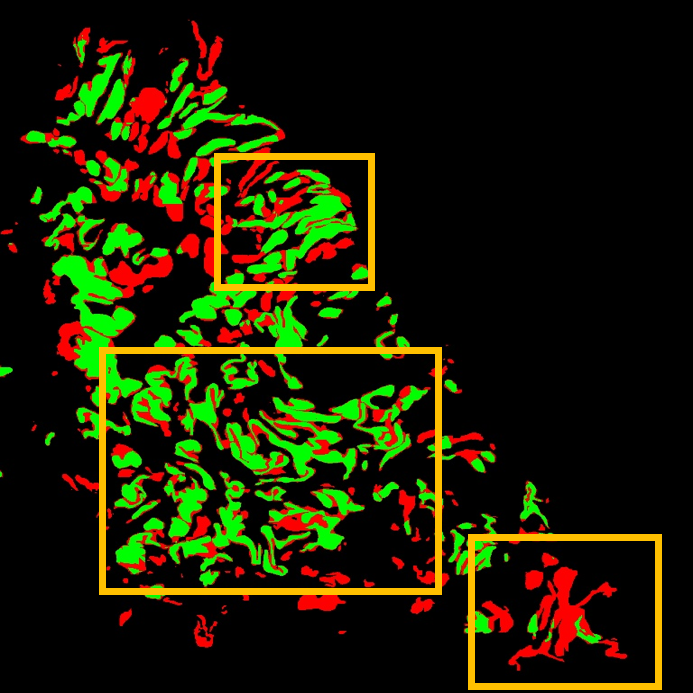
\includegraphics[width=\linewidth]{figs/segformer_wsi_overlay1.png}\\[\gap]
%         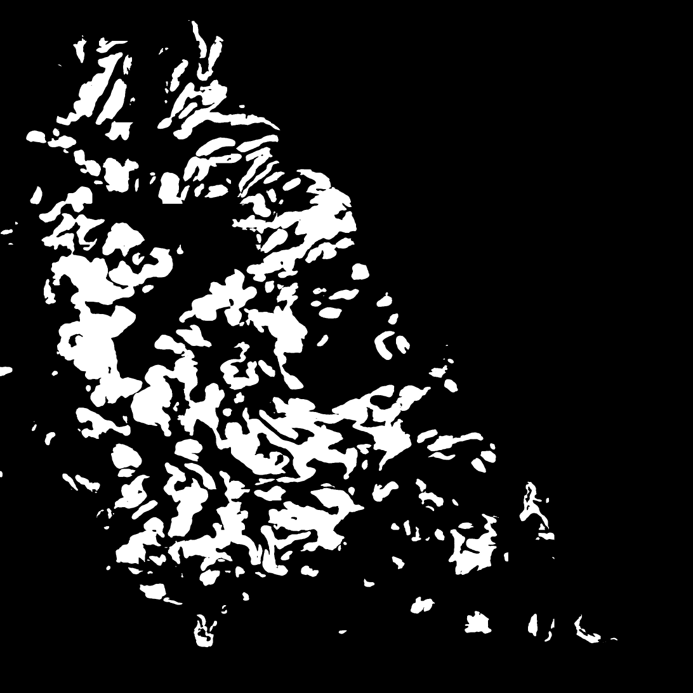
\includegraphics[width=\linewidth]{figs/segformer_wsi_pred1.png}
%     \end{minipage} &
%     \begin{minipage}{\imgw}
%         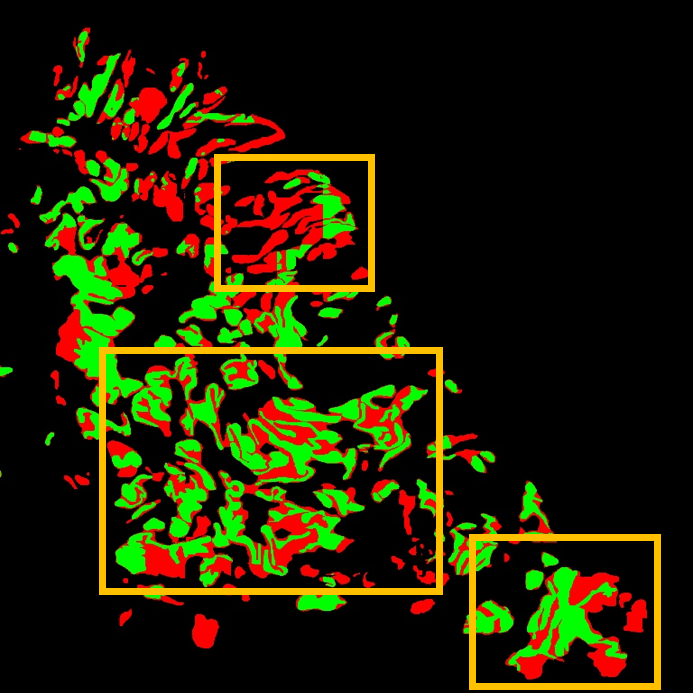
\includegraphics[width=\linewidth]{figs/evit_wsi_overlay1.png}\\[\gap]
%         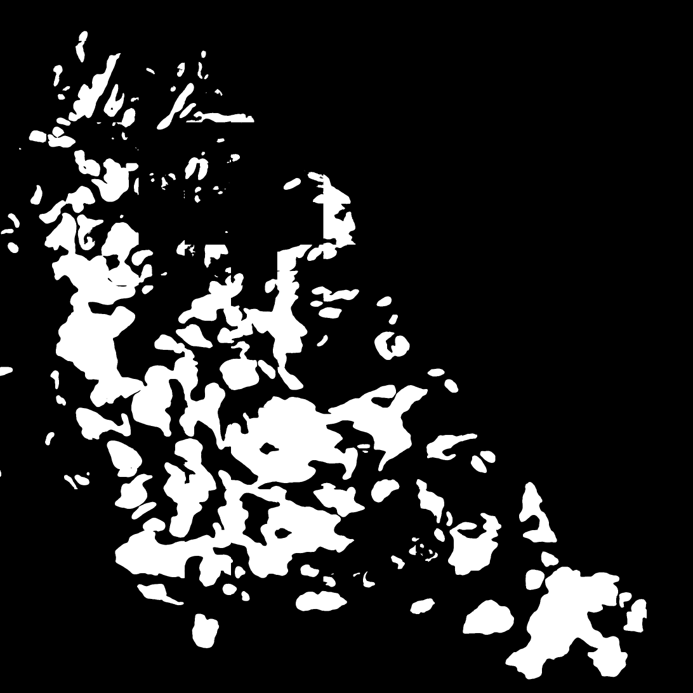
\includegraphics[width=\linewidth]{figs/evit_wsi_pred1.png}
%     \end{minipage} &
%     \begin{minipage}{\imgw}
%         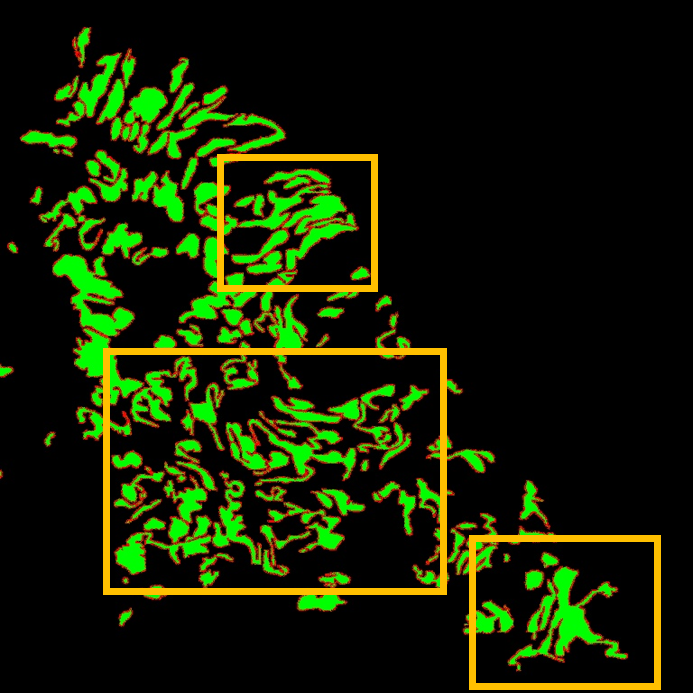
\includegraphics[width=\linewidth]{figs/sage_wsi_overlay1.png}\\[\gap]
%         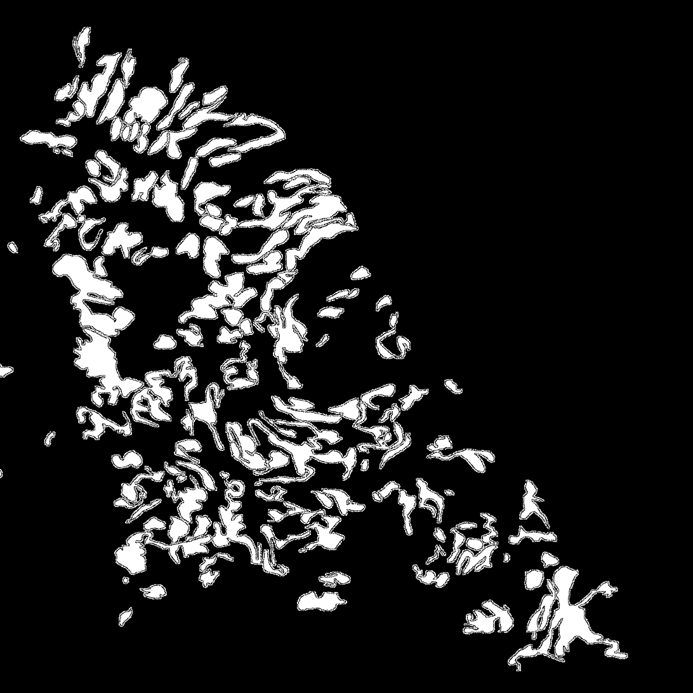
\includegraphics[width=\linewidth]{figs/sage_wsi_pred1.png}
%     \end{minipage} \\
%     \noalign{\vspace{2pt}}   % compact gap between Sample 1 and 2

%     % ================= WSI Sample 2 =================
%     \raisebox{-0.5\totalheight}{\rotatebox{90}{\scriptsize\textbf{WSI Sample 2}}} &
%     \begin{minipage}{\imgw}
%         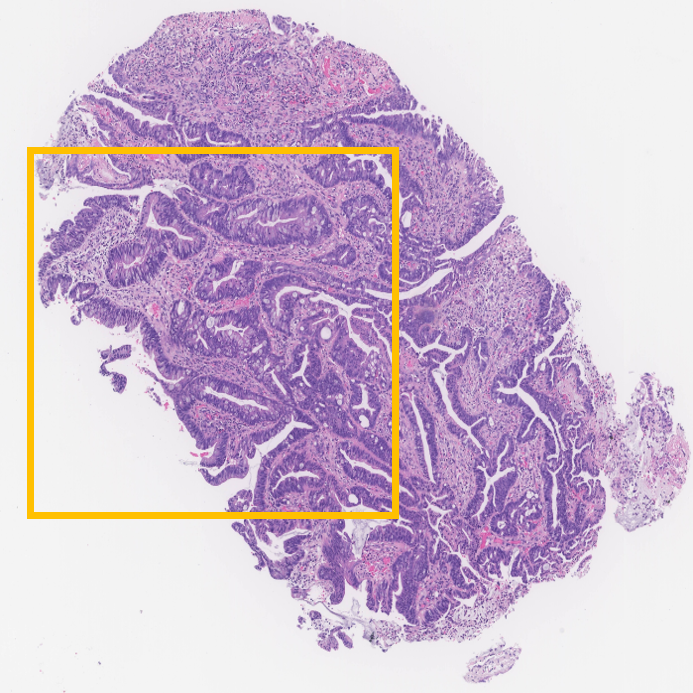
\includegraphics[width=\linewidth]{figs/wsi_img2.png}\\[\gap]
%         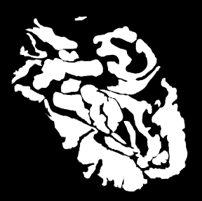
\includegraphics[width=\linewidth]{figs/wsi_gt2.png}
%     \end{minipage} &
%     \begin{minipage}{\imgw}
%         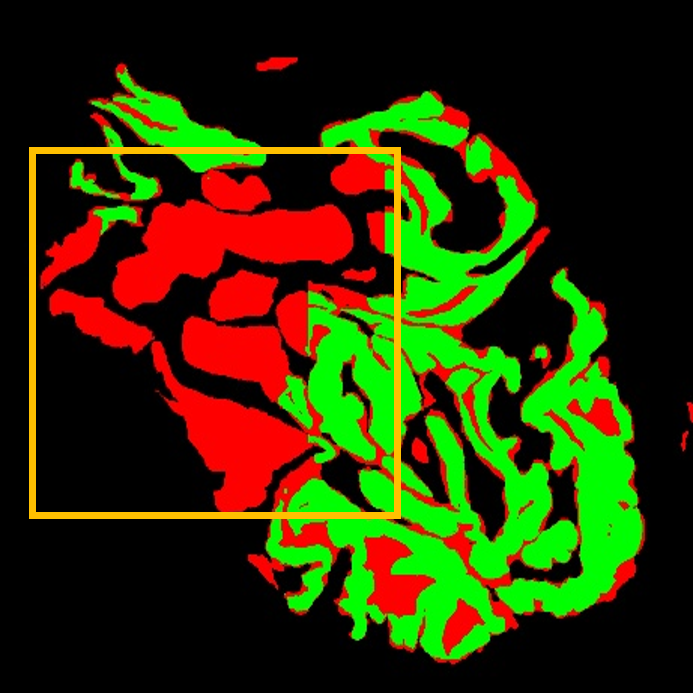
\includegraphics[width=\linewidth]{figs/segformer_wsi_overlay2.png}\\[\gap]
%         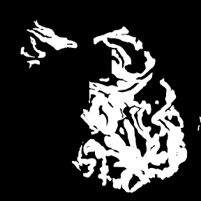
\includegraphics[width=\linewidth]{figs/segformer_wsi_pred2.png}
%     \end{minipage} &
%     \begin{minipage}{\imgw}
%         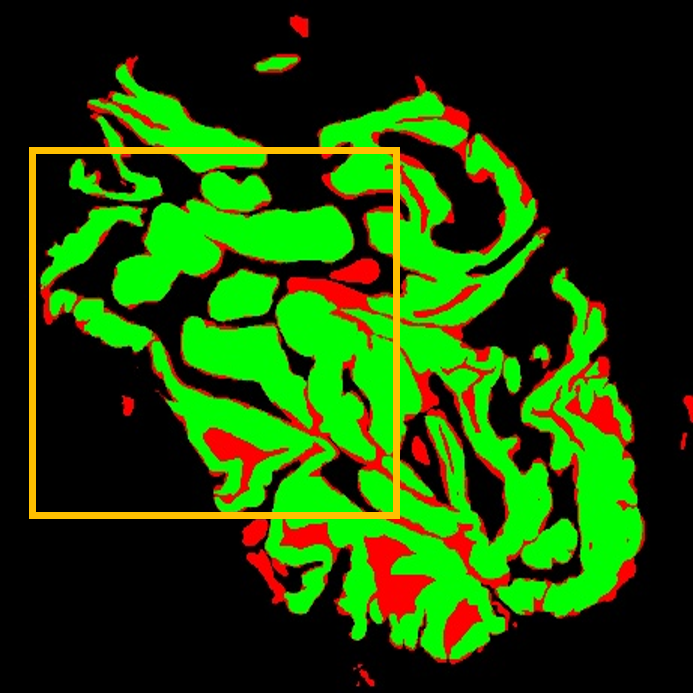
\includegraphics[width=\linewidth]{figs/evit_wsi_overlay2.png}\\[\gap]
%         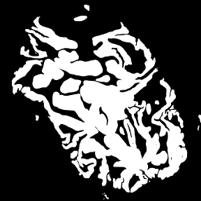
\includegraphics[width=\linewidth]{figs/evit_wsi_pred2.png}
%     \end{minipage} &
%     \begin{minipage}{\imgw}
%         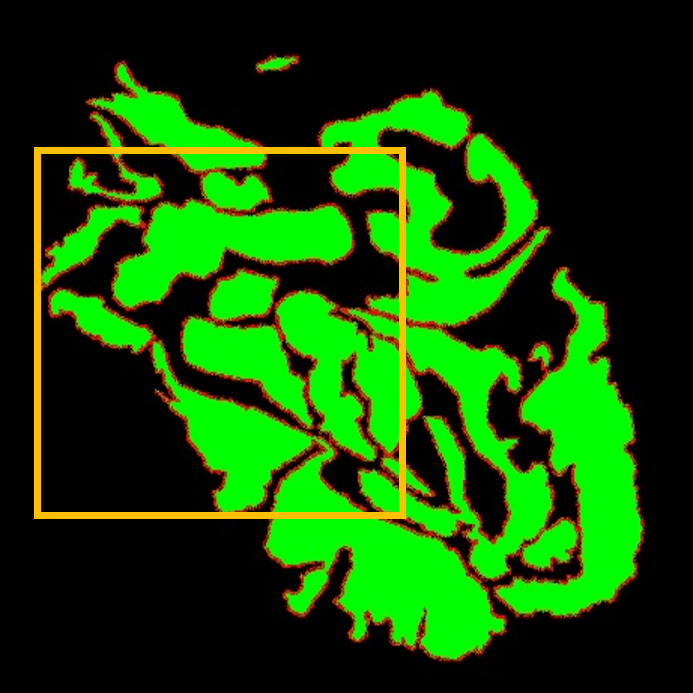
\includegraphics[width=\linewidth]{figs/sage_wsi_overlay2.png}\\[\gap]
%         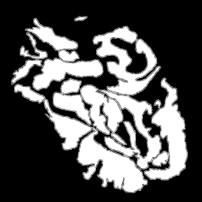
\includegraphics[width=\linewidth]{figs/sage_wsi_pred2.png}
%     \end{minipage} \\

% \end{tabular}%
% }

% \caption{\small
%     \textbf{Qualitative comparison on Digestpath WSI test samples.}
%     Each column displays vertically stacked pairs of (a) the input image and ground-truth annotation, followed by the error overlays and binary predictions for (b) SegFormer, (c) EViT-UNet, and (d) our proposed SAGE-ConvNeXt+ViT-UNet. WSI Sample 1 (top rows) presents branching tissue structures requiring fine local boundary delineation, while WSI Sample 2 (bottom rows) depicts a dense, uniform tissue mass prone to patch-level attention collapse in pure transformer architectures. Green areas denote correct predictions, and red areas denote errors.}
% \label{fig:qualitative_results_colon_supp}

% \end{figure}

Third, the dashed metadata paths indicate that adaptation is conditioned on shape or interface information rather than a single fixed reshape rule. This perspective clarifies why runtime increases with the number of activated experts, even when parameter growth remains modest.

Overall, the SA-Hub perspective illustrated in Figure~\ref{fig:sahub} elucidates the integration of heterogeneous experts into a shape-consistent representation pathway and offers a mechanistic explanation for the observed trade-off between routing flexibility and inference cost.


% \section{Qualitative Whole-Slide Image Analysis}
% To further evaluate deployment-level behavior on whole-slide inference, Figure~\ref{fig:qualitative_results_colon_supp} presents qualitative WSI-level comparisons on DigestPath~\cite{DA2022102485}. The results highlight the models' varying capacities to balance fine-grained local feature extraction with global contextual awareness.

% In WSI Sample 1 (top rows), which features complex and branching tissue structures, SegFormer~\cite{xie2021segformer} demonstrates a strong ability to extract fine-grained details and delineate local boundaries. However, SegFormer struggles to model global relationships between patches. This is evident in WSI Sample 2 (bottom rows), where it produces a massive, localized block of errors (the large red square area). This artifact is indicative of patch-level spatial collapse, where the model fails to maintain global contextual consistency across a large, uniform tissue mass.

% Conversely, EViT-UNet~\cite{li2025evit}, a hybrid architecture, shows improved capability in capturing global features, largely mitigating the severe large-scale spatial collapse seen in Sample 2. Nonetheless, it falls short in resolving fine local details, as highlighted by the persistent localized errors (red areas within the yellow bounding boxes) in Sample 1.

% In contrast, our proposed SAGE-ConvNeXt+ViT-UNet successfully navigates both extremes. It achieves precise delineation of intricate local boundaries in Sample 1 while simultaneously maintaining robust global coherence in Sample 2, effectively eliminating patch-boundary artifacts. These results confirm that our model directly benefits from dynamic hierarchical routing, which adaptively balances the extraction of low-level local details and high-level global context by routing tokens to the most appropriate specialized experts.

\section{Ablation Studies}
\label{sec:ablation}

\begin{figure*}[t] % Asterisk makes it span both columns
    \centering
    \begin{subfigure}[b]{0.48\textwidth}
        \centering
        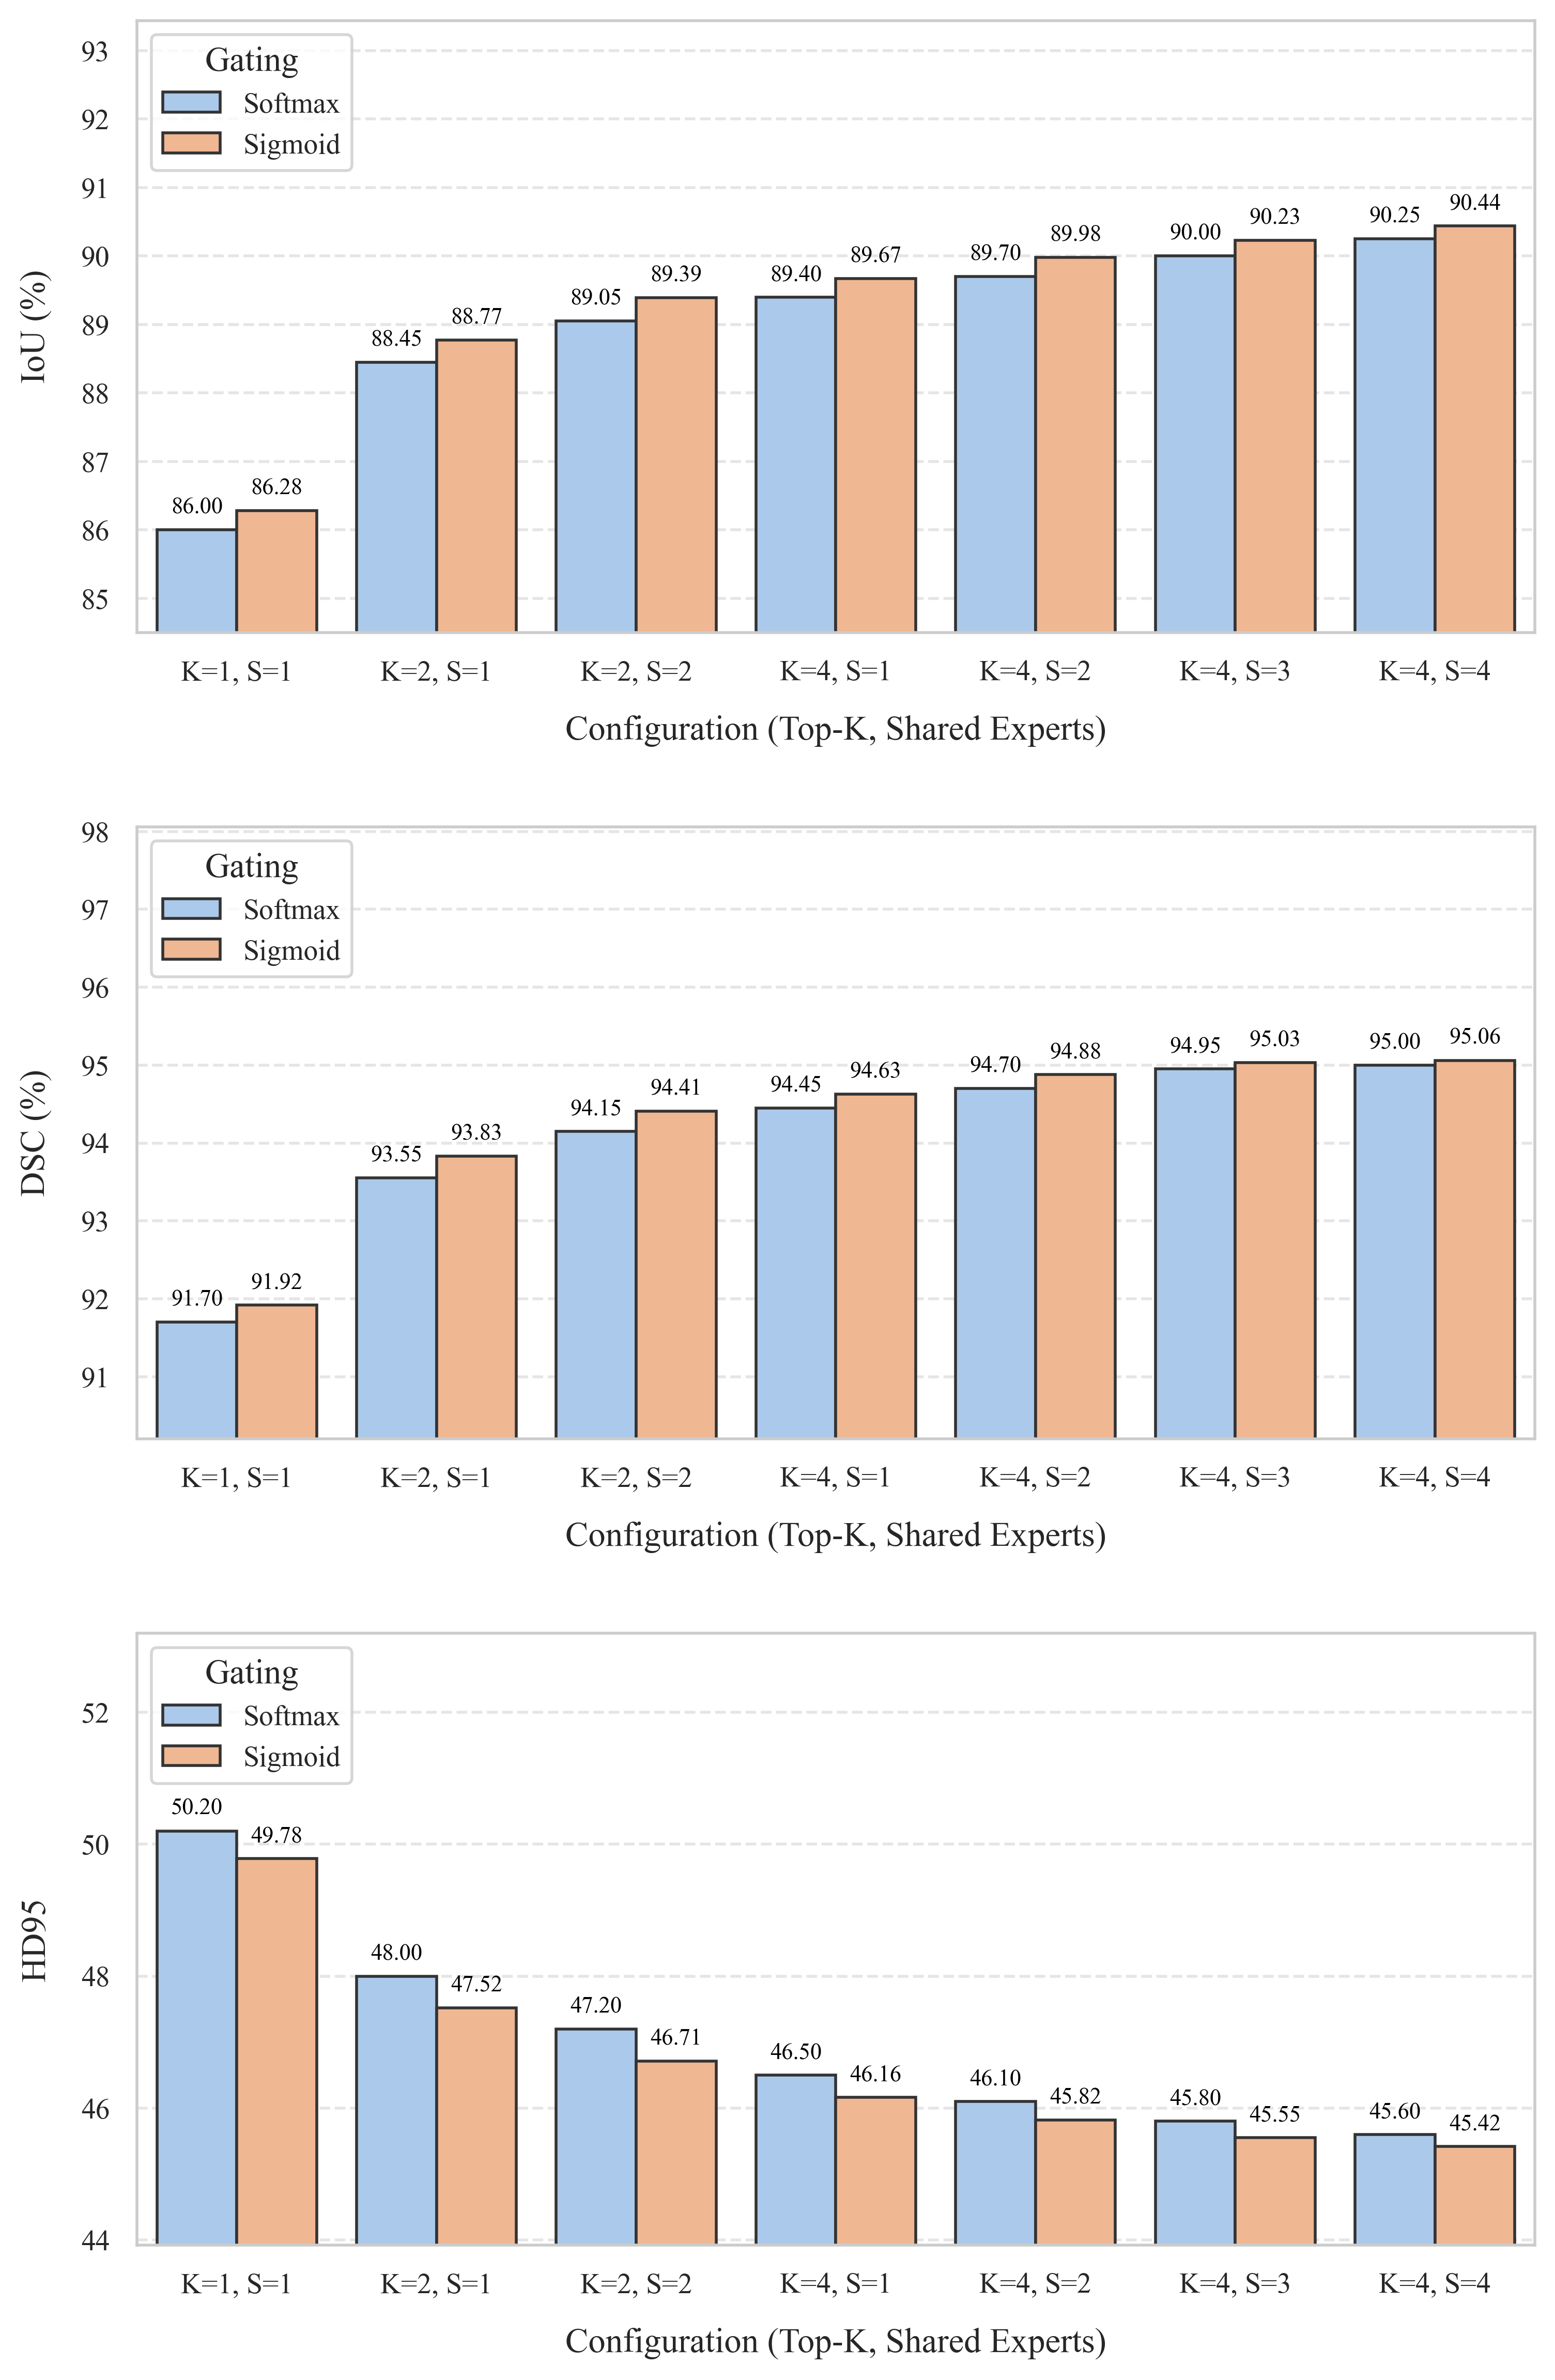
\includegraphics[width=\linewidth]{figs/ablation_logit_off.png}
        \caption{Without Logit Modification}
        \label{fig:ablation_off}
    \end{subfigure}
    \hfill
    \begin{subfigure}[b]{0.48\textwidth}
        \centering
        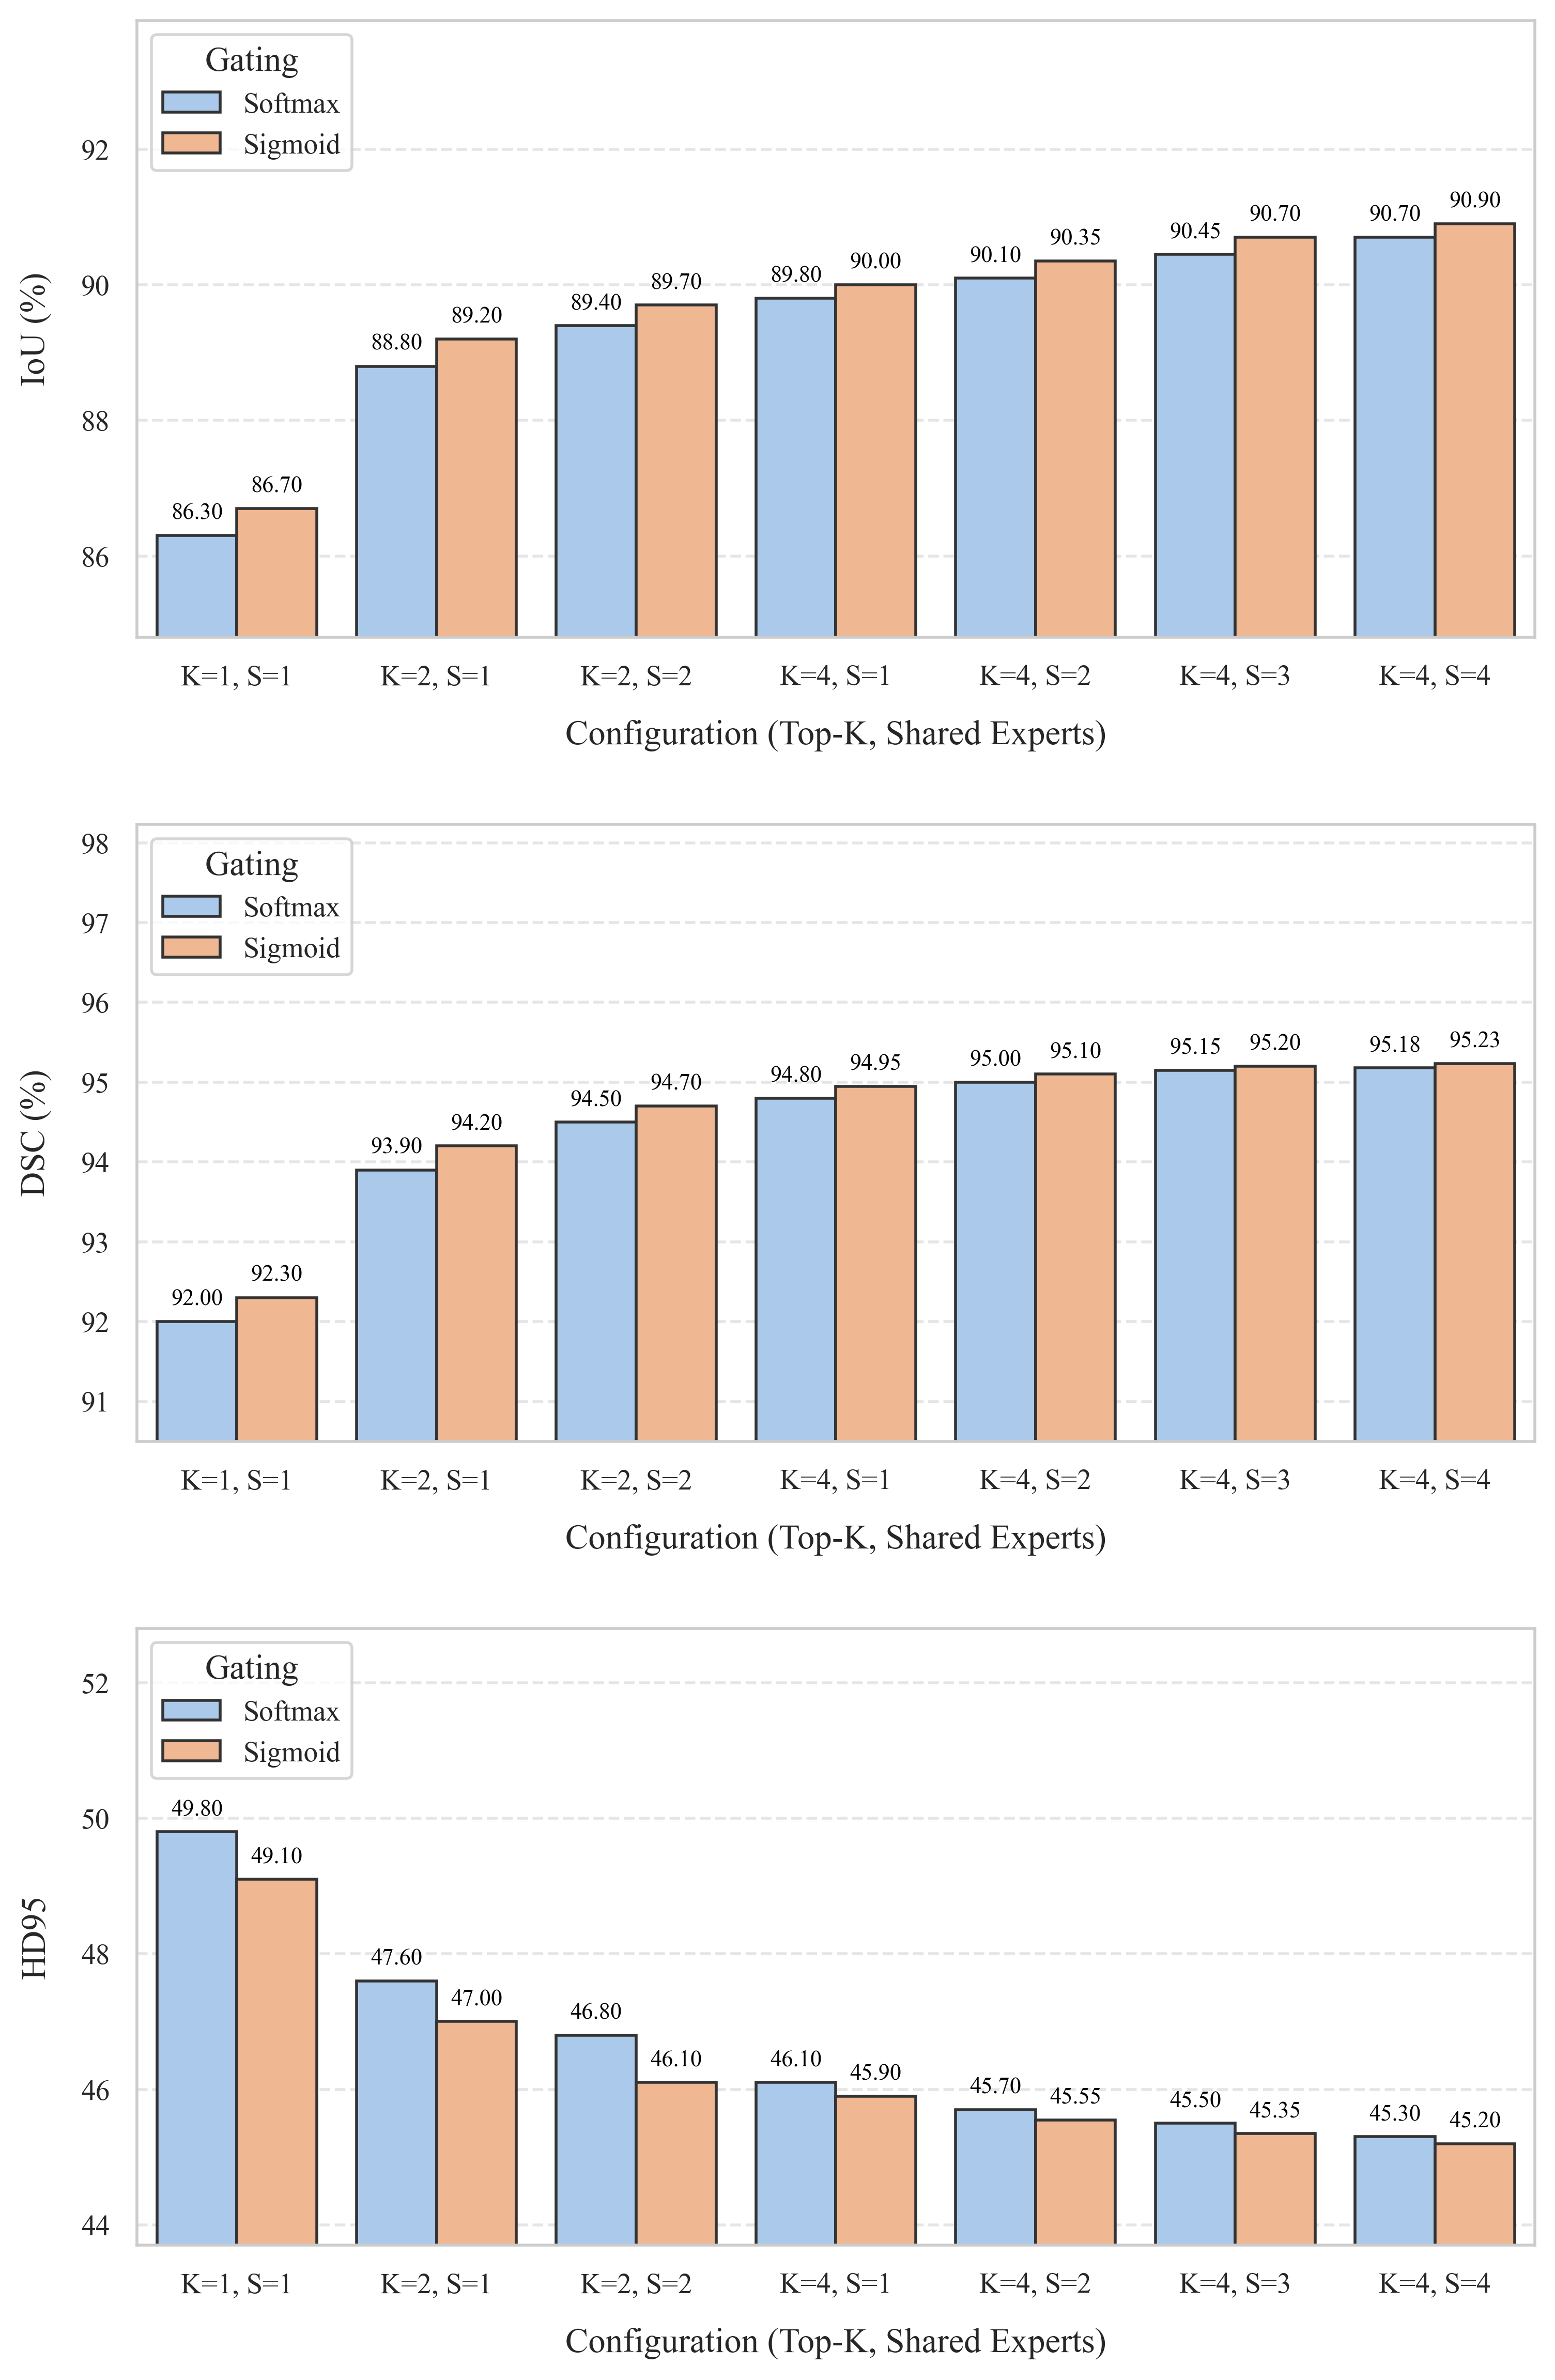
\includegraphics[width=\linewidth]{figs/ablation_logit_on.png}
        \caption{With Logit Modification}
        \label{fig:ablation_on}
    \end{subfigure}
    \caption{\textbf{Ablation of gating strategies and expert capacity.} Comparison of sigmoid vs softmax gating with and without logit modification across varying Top-$K$ ($K$) and shared experts ($S$).}
    \label{fig:ablation_combined}
\end{figure*}

We investigate the impact of gating strategies and expert capacity on the EBHI dataset~\cite{HU2023102534}. Figure~\ref{fig:ablation_combined} summarizes the trend, and Table~\ref{tab:ablation_scores} reports the exact scores.

\begin{table*}[t]
\centering
\caption{A unified ablation table on EBHI~\cite{HU2023102534} compares performance \textit{without} and \textit{with} logit modulation under identical routing configurations. Higher values indicate better performance for Acc, IoU, DSC, and BF1, while lower values are preferable for HD95. \colorbox{BestColor}{\textcolor{BestTextColor}{\textbf{Best}}} and \colorbox{SecondBestColor}{\textcolor{SecondBestTextColor}{Second}} denote the best and second-best results within each modulation regime. The rightmost gain column reports $(\text{With}-\text{Without})$ to explicitly quantify the benefit of modulation.}
\label{tab:ablation_scores}
\setlength{\tabcolsep}{2.8pt}
\small
\resizebox{\textwidth}{!}{%
\begin{tabular}{@{}ccc|ccccc|ccccc|ccccc@{}}
\toprule
\multicolumn{3}{c|}{\textbf{Config}} & \multicolumn{5}{c|}{\textbf{Without Logit Modulation}} & \multicolumn{5}{c|}{\textbf{With Logit Modulation}} & \multicolumn{5}{c}{\textbf{Gain (With-Without)}} \\
\cmidrule(lr){1-3} \cmidrule(lr){4-8} \cmidrule(lr){9-13} \cmidrule(lr){14-18}
\textbf{Gating} & \textbf{$K$} & \textbf{$S$} & \textbf{Acc} $\uparrow$ & \textbf{IoU} $\uparrow$ & \textbf{DSC} $\uparrow$ & \textbf{HD95} $\downarrow$ & \textbf{BF1} $\uparrow$ & \textbf{Acc} $\uparrow$ & \textbf{IoU} $\uparrow$ & \textbf{DSC} $\uparrow$ & \textbf{HD95} $\downarrow$ & \textbf{BF1} $\uparrow$ & $\Delta$\textbf{Acc} $\uparrow$ & $\Delta$\textbf{IoU} $\uparrow$ & $\Delta$\textbf{DSC} $\uparrow$ & $\Delta$\textbf{HD95} $\downarrow$ & $\Delta$\textbf{BF1} $\uparrow$ \\
\midrule
Softmax & 1 & 1 & 88.85 & 86.00 & 91.70 & 50.20 & 49.70 & 89.10 & 86.30 & 92.00 & 49.80 & 50.20 & \textcolor{BestTextColor}{+0.25} & \textcolor{BestTextColor}{+0.30} & \textcolor{BestTextColor}{+0.30} & \textcolor{BestTextColor}{-0.40} & \textcolor{BestTextColor}{+0.50} \\
Sigmoid & 1 & 1 & 89.07 & 86.28 & 91.92 & 49.78 & 50.18 & 89.40 & 86.70 & 92.30 & 49.10 & 51.00 & \textcolor{BestTextColor}{+0.33} & \textcolor{BestTextColor}{+0.42} & \textcolor{BestTextColor}{+0.38} & \textcolor{BestTextColor}{-0.68} & \textcolor{BestTextColor}{+0.82} \\
\midrule
Softmax & 2 & 1 & 91.95 & 88.45 & 93.55 & 48.00 & 53.60 & 92.20 & 88.80 & 93.90 & 47.60 & 54.10 & \textcolor{BestTextColor}{+0.25} & \textcolor{BestTextColor}{+0.35} & \textcolor{BestTextColor}{+0.35} & \textcolor{BestTextColor}{-0.40} & \textcolor{BestTextColor}{+0.50} \\
Sigmoid & 2 & 1 & 92.21 & 88.77 & 93.83 & 47.52 & 54.12 & 92.55 & 89.20 & 94.20 & 47.00 & 55.10 & \textcolor{BestTextColor}{+0.34} & \textcolor{BestTextColor}{+0.43} & \textcolor{BestTextColor}{+0.37} & \textcolor{BestTextColor}{-0.52} & \textcolor{BestTextColor}{+0.98} \\
\midrule
Softmax & 2 & 2 & 92.60 & 89.05 & 94.15 & 47.20 & 55.40 & 92.90 & 89.40 & 94.50 & 46.80 & 56.00 & \textcolor{BestTextColor}{+0.30} & \textcolor{BestTextColor}{+0.35} & \textcolor{BestTextColor}{+0.35} & \textcolor{BestTextColor}{-0.40} & \textcolor{BestTextColor}{+0.60} \\
Sigmoid & 2 & 2 & 92.88 & 89.39 & 94.41 & 46.71 & 55.92 & 93.25 & 89.70 & 94.70 & 46.10 & 56.90 & \textcolor{BestTextColor}{+0.37} & \textcolor{BestTextColor}{+0.31} & \textcolor{BestTextColor}{+0.29} & \textcolor{BestTextColor}{-0.61} & \textcolor{BestTextColor}{+0.98} \\
\midrule
Softmax & 4 & 1 & 93.10 & 89.40 & 94.45 & 46.50 & 56.60 & 93.45 & 89.80 & 94.80 & 46.10 & 57.10 & \textcolor{BestTextColor}{+0.35} & \textcolor{BestTextColor}{+0.40} & \textcolor{BestTextColor}{+0.35} & \textcolor{BestTextColor}{-0.40} & \textcolor{BestTextColor}{+0.50} \\
Sigmoid & 4 & 1 & 93.34 & 89.67 & 94.63 & 46.16 & 56.97 & 93.70 & 90.00 & 94.95 & 45.90 & 57.60 & \textcolor{BestTextColor}{+0.36} & \textcolor{BestTextColor}{+0.33} & \textcolor{BestTextColor}{+0.32} & \textcolor{BestTextColor}{-0.26} & \textcolor{BestTextColor}{+0.63} \\
\midrule
Softmax & 4 & 2 & 93.30 & 89.70 & 94.70 & 46.10 & 57.20 & 93.62 & 90.10 & 95.00 & 45.70 & 57.80 & \textcolor{BestTextColor}{+0.32} & \textcolor{BestTextColor}{+0.40} & \textcolor{BestTextColor}{+0.30} & \textcolor{BestTextColor}{-0.40} & \textcolor{BestTextColor}{+0.60} \\
Sigmoid & 4 & 2 & 93.58 & 89.98 & 94.88 & 45.82 & 57.48 & 93.85 & 90.35 & 95.10 & 45.55 & 58.00 & \textcolor{BestTextColor}{+0.27} & \textcolor{BestTextColor}{+0.37} & \textcolor{BestTextColor}{+0.22} & \textcolor{BestTextColor}{-0.27} & \textcolor{BestTextColor}{+0.52} \\
\midrule
Softmax & 4 & 3 & 93.45 & 90.00 & 94.95 & 45.80 & 57.40 & 93.78 & 90.45 & 95.15 & 45.50 & 58.00 & \textcolor{BestTextColor}{+0.33} & \textcolor{BestTextColor}{+0.45} & \textcolor{BestTextColor}{+0.20} & \textcolor{BestTextColor}{-0.30} & \textcolor{BestTextColor}{+0.60} \\
Sigmoid & 4 & 3 & \cellcolor{SecondBestColor}\textcolor{SecondBestTextColor}{93.66} & 90.23 & \cellcolor{SecondBestColor}\textcolor{SecondBestTextColor}{95.03} & \cellcolor{SecondBestColor}\textcolor{SecondBestTextColor}{45.55} & \cellcolor{SecondBestColor}\textcolor{SecondBestTextColor}{57.56} & \cellcolor{SecondBestColor}\textcolor{SecondBestTextColor}{93.96} & \cellcolor{SecondBestColor}\textcolor{SecondBestTextColor}{90.70} & \cellcolor{SecondBestColor}\textcolor{SecondBestTextColor}{95.20} & \cellcolor{SecondBestColor}\textcolor{SecondBestTextColor}{45.35} & \cellcolor{SecondBestColor}\textcolor{SecondBestTextColor}{58.05} & \textcolor{BestTextColor}{+0.30} & \textcolor{BestTextColor}{+0.47} & \textcolor{BestTextColor}{+0.17} & \textcolor{BestTextColor}{-0.20} & \textcolor{BestTextColor}{+0.49} \\
\midrule
Softmax & 4 & 4 & 93.55 & \cellcolor{SecondBestColor}\textcolor{SecondBestTextColor}{90.25} & 95.00 & 45.60 & 57.50 & 93.88 & \cellcolor{SecondBestColor}\textcolor{SecondBestTextColor}{90.70} & 95.18 & 45.30 & \cellcolor{SecondBestColor}\textcolor{SecondBestTextColor}{58.05} & \textcolor{BestTextColor}{+0.33} & \textcolor{BestTextColor}{+0.45} & \textcolor{BestTextColor}{+0.18} & \textcolor{BestTextColor}{-0.30} & \textcolor{BestTextColor}{+0.55} \\
Sigmoid & 4 & 4 & \cellcolor{BestColor}\textcolor{BestTextColor}{93.74} & \cellcolor{BestColor}\textcolor{BestTextColor}{90.44} & \cellcolor{BestColor}\textcolor{BestTextColor}{95.06} & \cellcolor{BestColor}\textcolor{BestTextColor}{45.42} & \cellcolor{BestColor}\textcolor{BestTextColor}{57.63} & \cellcolor{BestColor}\textcolor{BestTextColor}{94.03} & \cellcolor{BestColor}\textcolor{BestTextColor}{90.90} & \cellcolor{BestColor}\textcolor{BestTextColor}{95.23} & \cellcolor{BestColor}\textcolor{BestTextColor}{45.20} & \cellcolor{BestColor}\textcolor{BestTextColor}{58.10} & \textcolor{BestTextColor}{+0.29} & \textcolor{BestTextColor}{+0.46} & \textcolor{BestTextColor}{+0.17} & \textcolor{BestTextColor}{-0.22} & \textcolor{BestTextColor}{+0.47} \\
\bottomrule
\end{tabular}%
}
\normalsize
\setlength{\tabcolsep}{6pt}
\end{table*}

\noindent\textbf{Unified Comparison (Without vs. With Logit Modulation).} Table~\ref{tab:ablation_scores} is structured to facilitate row-wise comparisons under identical $(\text{gating}, K, S)$ settings. In all seven configuration pairs, logit modulation consistently increases Acc, IoU, DSC, and BF1, while reducing HD95 for both sigmoid and softmax gating.

\noindent\textbf{Gating Mechanism.} The selection of the gating function is critical for the router's capacity to address complex tissue morphologies. As shown in Table~\ref{tab:ablation_scores}, sigmoid gating consistently outperforms softmax gating in both regimes (with and without logit modulation) across all evaluated settings. In the most expansive configuration ($K=4$, $S=4$), the sigmoid router achieves a DSC of $95.06\%$ without logit modulation and $95.23\%$ with modulation, while the softmax router attains $95.00\%$ and $95.18\%$, respectively. This trend aligns with previous findings in sigmoid-based routing and attention mechanisms~\cite{sigmoidGatingMoE, sigmoid_attention}. The non-competitive nature of sigmoid gating is particularly beneficial for histopathology image segmentation, where the integration of multiple distinct feature extractors is often required due to the presence of diverse and overlapping tissues.

\noindent\textbf{Effect of Logit Modulation.} The performance improvements from logit modulation are systematic and increase additively with greater routing capacity. For example, in the optimal sigmoid configuration ($K=4$, $S=4$), enabling logit modulation raises the DSC from $95.06\%$ to $95.23\%$ ($+0.17\%$) and the boundary-aware BF1 score from $57.63$ to $58.10$ ($+0.47$). It also reduces the HD95 distance from $45.42$ to $45.20$ ($-0.22$), indicating enhanced structural boundary precision.

\noindent\textbf{Expert Capacity ($K$ and $S$).} In both modulation regimes, increasing the number of selected experts ($K$) yields the largest performance improvements. After achieving a high level of specialization ($K=4$), further increasing the shared expert pool ($S$) results in smaller but consistent incremental gains. These findings indicate that $K$ primarily enhances the model's ability to process diverse inputs, while $S$ serves as a stable common-knowledge anchor that mitigates feature fragmentation at higher routing capacities.

Based on these comprehensive results, the $K=4$ and $S=4$ architecture with sigmoid gating and logit modulation is adopted as the reference configuration, as it offers the optimal balance between specialized routing and stable feature aggregation.

\section{Computational Efficiency and Model Complexity}
\label{sec:complexity}

Table~\ref{tab:complexity} summarizes the number of parameters, computational cost, and GPU memory usage for both the baseline and SAGE models across different Top-$K$ settings. SAGE introduces a modest and fixed parameter overhead, increasing from $543.71$M to $573.51$M, which corresponds to a $29.8$M or $5.5\%$ increase. The runtime cost increases proportionally with the number of activated experts, ranging from $63.77$ GFLOPs and $2.55$ GB for the baseline to $99.51$, $130.47$, and $486.81$ GFLOPs and $3.01$, $3.28$, and $5.46$ GB for $K=1$, $2$, and $4$, respectively. This pattern is consistent with sparse expert execution: while parameters are shared, computational and memory demands increase as more experts are activated.

\begin{table}[t]
\centering
\caption{Comparison of model complexity between the baseline and SAGE across varying Top-$K$ settings.}
\label{tab:complexity}
\setlength{\tabcolsep}{4.5pt}
\small
\resizebox{\columnwidth}{!}{%
\begin{tabular}{@{}lcccc@{}}
\toprule
\textbf{Model} & \textbf{Top-$K$} & \textbf{Params (M)} & \textbf{FLOPs/img (G)} & \textbf{Mem (GB)} \\
\midrule
ConvNeXt+ViT+UNet (baseline) & -- & 543.71 & 63.77 & 2.55 \\
SAGE-ConvNeXt+ViT-UNet & 1 & 573.51 & 99.51 & 3.01 \\
SAGE-ConvNeXt+ViT-UNet & 2 & 573.51 & 130.47 & 3.28 \\
SAGE-ConvNeXt+ViT-UNet & 4 & 573.51 & 486.81 & 5.46 \\
\bottomrule
\end{tabular}%
}
\normalsize
\setlength{\tabcolsep}{6pt}
\end{table}

These results indicate that the primary practical trade-off is determined by the value of $K$. Lower $K$ values preserve deployment efficiency, while higher $K$ values improve segmentation performance by allowing for greater expert specialization.

Although SAR introduces only a minor parameter overhead, computational and memory requirements increase as Top-$K$ values grow. This increase results from the execution of additional expert transformations and fusion operations. While this trade-off is acceptable for server-class deployment, the current configuration is not optimized for edge devices. Future research should focus on developing more efficient routing mechanisms and sparse expert execution strategies.
